% Local Taylor polynomials of sine on [0,1.05], with the point x=0.1 marked.
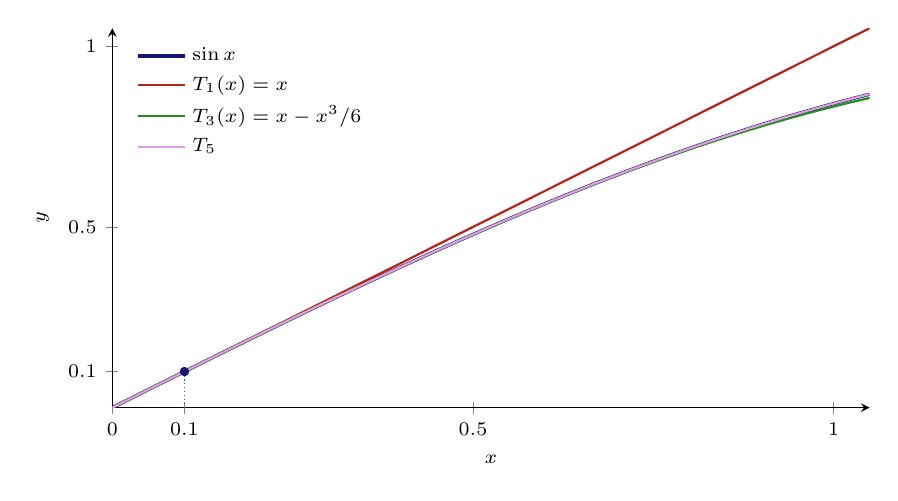
\begin{tikzpicture}
\begin{axis}[width=11.2cm,height=6.4cm,xmin=0,xmax=1.05,ymin=0,ymax=1.05,axis lines=left,xlabel={$x$},ylabel={$y$},xtick={0,0.1,0.5,1},ytick={0.1,0.5,1},tick label style={font=\scriptsize},label style={font=\scriptsize},legend style={font=\scriptsize,at={(0.02,0.98)},anchor=north west,draw=none,fill=none},legend cell align={left}]
  \addplot[MidnightBlue,very thick,domain=0:1.05,samples=80] {sin(deg(x))};
  \addlegendentry{$\sin x$}
  \addplot[BrickRed,thick,domain=0:1.05,samples=40] {x};
  \addlegendentry{$T_1(x)=x$}
  \addplot[ForestGreen,thick,domain=0:1.05,samples=50] {x-x^3/6};
  \addlegendentry{$T_3(x)=x-x^3/6$}
  \addplot[Plum,thick,domain=0:1.05,samples=60] {x-x^3/6+x^5/120};
  \addlegendentry{$T_5$}
  \draw[densely dotted,teal] (axis cs:0.1,0) -- (axis cs:0.1,{sin(deg(0.1))});
  \addplot[MidnightBlue,only marks,mark=*,mark size=1.5pt] coordinates {(0.1,0.099833)};
\end{axis}
\end{tikzpicture}
